\documentclass[journal]{IEEETemplate/IEEEtran}


\usepackage[english]{babel}



% *** CITATION PACKAGES ***
%
\usepackage{cite}


% *** MATH PACKAGES ***
%
\usepackage[cmex10]{amsmath}

\interdisplaylinepenalty=2500


% *** ALIGNMENT PACKAGES ***
%
\usepackage{array}

% *** FLOAT PACKAGES ***
%
\usepackage{fixltx2e}
\usepackage{float}

\usepackage{stfloats}


% *** PDF, URL AND HYPERLINK PACKAGES ***
%
\usepackage{url}
\usepackage[pdftex]{graphicx}



\begin{document}
%
% paper title
% Titles are generally capitalized except for words such as a, an, and, as,
% at, but, by, for, in, nor, of, on, or, the, to and up, which are usually
% not capitalized unless they are the first or last word of the title.
% Linebreaks \\ can be used within to get better formatting as desired.
% Do not put math or special symbols in the title.
\title{Neural Sequence Embedding generalization with Density-Based Clustering}
%
%
% author names and IEEE memberships
% note positions of commas and nonbreaking spaces ( ~ ) LaTeX will not break
% a structure at a ~ so this keeps an author's name from being broken across
% two lines.
% use \thanks{} to gain access to the first footnote area
% a separate \thanks must be used for each paragraph as LaTeX2e's \thanks
% was not built to handle multiple paragraphs
%

\author{Milan van der Meer}% <-this % stops a space




% The paper headers
\markboth{}%
{Neural Sequence Embedding generalization with Density-Based Clustering}
% The only time the second header will appear is for the odd numbered pages
% after the title page when using the twoside option.
% 
% *** Note that you probably will NOT want to include the author's ***
% *** name in the headers of peer review papers.                   ***
% You can use \ifCLASSOPTIONpeerreview for conditional compilation here if
% you desire.



% make the title area
\maketitle

% As a general rule, do not put math, special symbols or citations
% in the abstract or keywords.
\begin{abstract}
Large medical databases give the opportunity to build models for predicting the disease progression of a patient. To build the model, preprocessing of the data is necessary. We introduce a method based on word2vec applied on complex states. Before applying word2vec, it is possible to apply DBSCAN clustering to receive more general results without ignoring medical outliers. It is too early to draw a conclusion on the effects of those methods.
\end{abstract}

% Note that keywords are not normally used for peerreview papers.
\begin{IEEEkeywords}
Embedding, clustering, LSTM
\end{IEEEkeywords}






% For peer review papers, you can put extra information on the cover
% page as needed:
% \ifCLASSOPTIONpeerreview
% \begin{center} \bfseries EDICS Category: 3-BBND \end{center}
% \fi
%
% For peerreview papers, this IEEEtran command inserts a page break and
% creates the second title. It will be ignored for other modes.
\IEEEpeerreviewmaketitle



\section{Motivation}

\IEEEPARstart{O}{ne} of the prerequisites for precision medication is predicting the disease progression of a patient. Often medical datasets are researched with a limited amount of data or with simple machine learning techniques. This paper introduces the first part of a larger work in which advanced machine learning techniques are applied on a large-scale medical dataset. This paper focuses on the preprocessing of the data before it is fed into a Neural Network. \\
In medical data there is a large amount of attributes which causes a large amount of possible events. Because of this, most events are unique. To get a more general model, those distinct events should be generalized. One of the problems with medical data is that outliers in the data need special attention because those could potentially be valuable. In short, there is a need for a method which generalizes the data but still gives special attention to outliers. \\
As mentioned before, we have a lot of different attributes which causes our data to be sparse. We could try to represent the data in a more dense space. We can use the sequences of a patients states to find relations between the states. The relations can be represented in the denser space by putting the states related to each other close in the new space. Using this representation, Neural Networks can be trained better. \\
Because the states are very distinct, the probability that a completely new state needs to be predicted by the found model is quite high. Our final method should be able to handle this.
 
\hfill December 30, 2015



\section{Previous Research}
Embedding is a well researched topic in the area of protein sequences\cite{1,2} and natural language processing\cite{3,4}. Embedding applied on medical data is as far as our knowledge goes, not done before. The area where complex sequences are embedded is also limited. \\
Clustering is a popular method in the medical field\cite{5,6}. But the combination with our embedding method isn't done before as far as our knowledge goes. \\


\section{Problem Definition}
In this section we describe our problem and each of the subproblems. We describe more general problems which occur in large datasets and some more specific problems related to the prediction method. \\

The medical history of a patient is a time series with each medical status a data point in time. The main goal is to predict a label for each time series. For example: patient will be cured. To achieve this goal, we need to preprocess the data before we apply a prediction method onto it. \\
A high dimensional numerical vector represents a medical status where a value can express for example the blood pressure of a patient. Between data points, there can be long time periods and also irregular intervals. The numerical values of the vectors need to be standardized. Typical for large datasets, are missing values which have to be taken into account. \\

\subsubsection{Time Series}
Each patient is an independent time series. But in the time series, several independent disease periods can occur. In medical data, there are a large amount of unique events because of the high dimensional data points. Each possible combination of the vector space represents an unique event. Machine learning techniques are harder to apply when there are a large amount of different events\cite{7}, especially when rare events are possibly important which is the case in medical data\cite{8}. \\
\subsubsection{Long Time Periods}
\label{sec:LongTimePeriods}
Between the events are a long range of dependencies possible. When machine learning techniques try to model those dependencies, a decay or blow up of events can happen, this is called the vanishing gradient problem\cite{9}. \\
\subsubsection{Irregular Intervals}
\label{sec:IrregularIntervals}
Irregular intervals are a form of missing data. Our method has to handle the irregular intervals or transform them accordingly to regular intervals\cite{10}. \\
\subsubsection{High Dimensionality}
\label{sec:HighDimensionality}
A well known problem is the Curse of Dimensionality\cite{11}. It causes the data to be sparse and implies the need for more data. Also the effects and importance of attributes is unclear because of the large amount of attributes. \\
\subsubsection{Sequence Labeling}
Our prediction method should handle all above mentioned problems and be able to build a model to label a given sequence. The label is an indicator on what the outcome will be of the patients disease trajectory. The labeling process gives the prediction of the disease trajectory. \\
Sequence labeling can be done with Recurrent Neural Networks (RNN). A RNN which handles problems like \ref{sec:LongTimePeriods}, \ref{sec:IrregularIntervals}, and \ref{sec:HighDimensionality} is Long Short Term Memory (LSTM)\cite{12}. \\
\subsubsection{Embedding} 
Because of the sparse structure of the data, it would be ideal to transform the data to a more compact presentation. This process is called embedding\cite{13a}. Embedding also tries to find relations between the original data and represent those relations by projecting the related data points closely in the projection space. The embedding can be used to feed into a LSTM network. \\

The method described in \ref{sec:Methods} tries to handle the preprocessing needed for the LSTM network.

\section{Methods}
\label{sec:Methods}
We first describe our approach on the problems as irregular intervals and normalization. Secondly, we describe our method to make the embedding matrix. Lastly, we introduce a method to generalize our events to get a more general embedding matrix but still keep outliers.

\subsection{Preprocessing}
The irregular intervals are mainly ignored as they don't effect the preprocessing. The events get a new attribute to directly specify the length of the interval between the current event and the previous event. This way the time difference is added explicitly to the data. The normalization is done for the purpose of clustering because we don't want to make any assumption on the importance of any attribute\cite{14}. The embedding is done without normalization but it could be applied also\cite{15}. For the normalization we make the data Gaussian with zero mean and unit variance.

\subsection{Embedding}
Embedding is done based on the word2vec approach\cite{13}. It is a two-layer neural network which encodes words in vectors. They use a skip-gram model to predict a context when a word is given. The model will make the representation space less sparse and also locate words related to each other closely in this new space.

\begin{figure}[H]
\centering
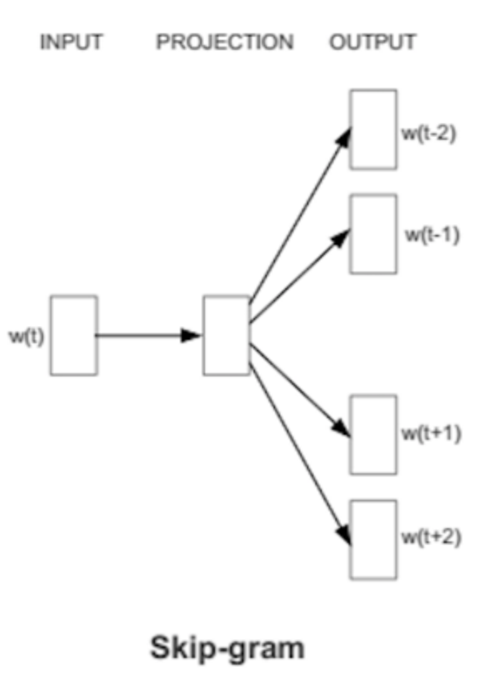
\includegraphics[width=2.5in]{../Figures/skipGram.pdf}
\caption{Skip-Gram model}
\label{fig:skipgram}
\end{figure}

The same can be applied on more complex states than words. We first order all our sequences chronology and put them into one text file. Each sequence is separated by some label so there are no relations found between the start and the end of two different sequences. We apply the word2vec method on this text file. 

\begin{figure}[H]
\centering
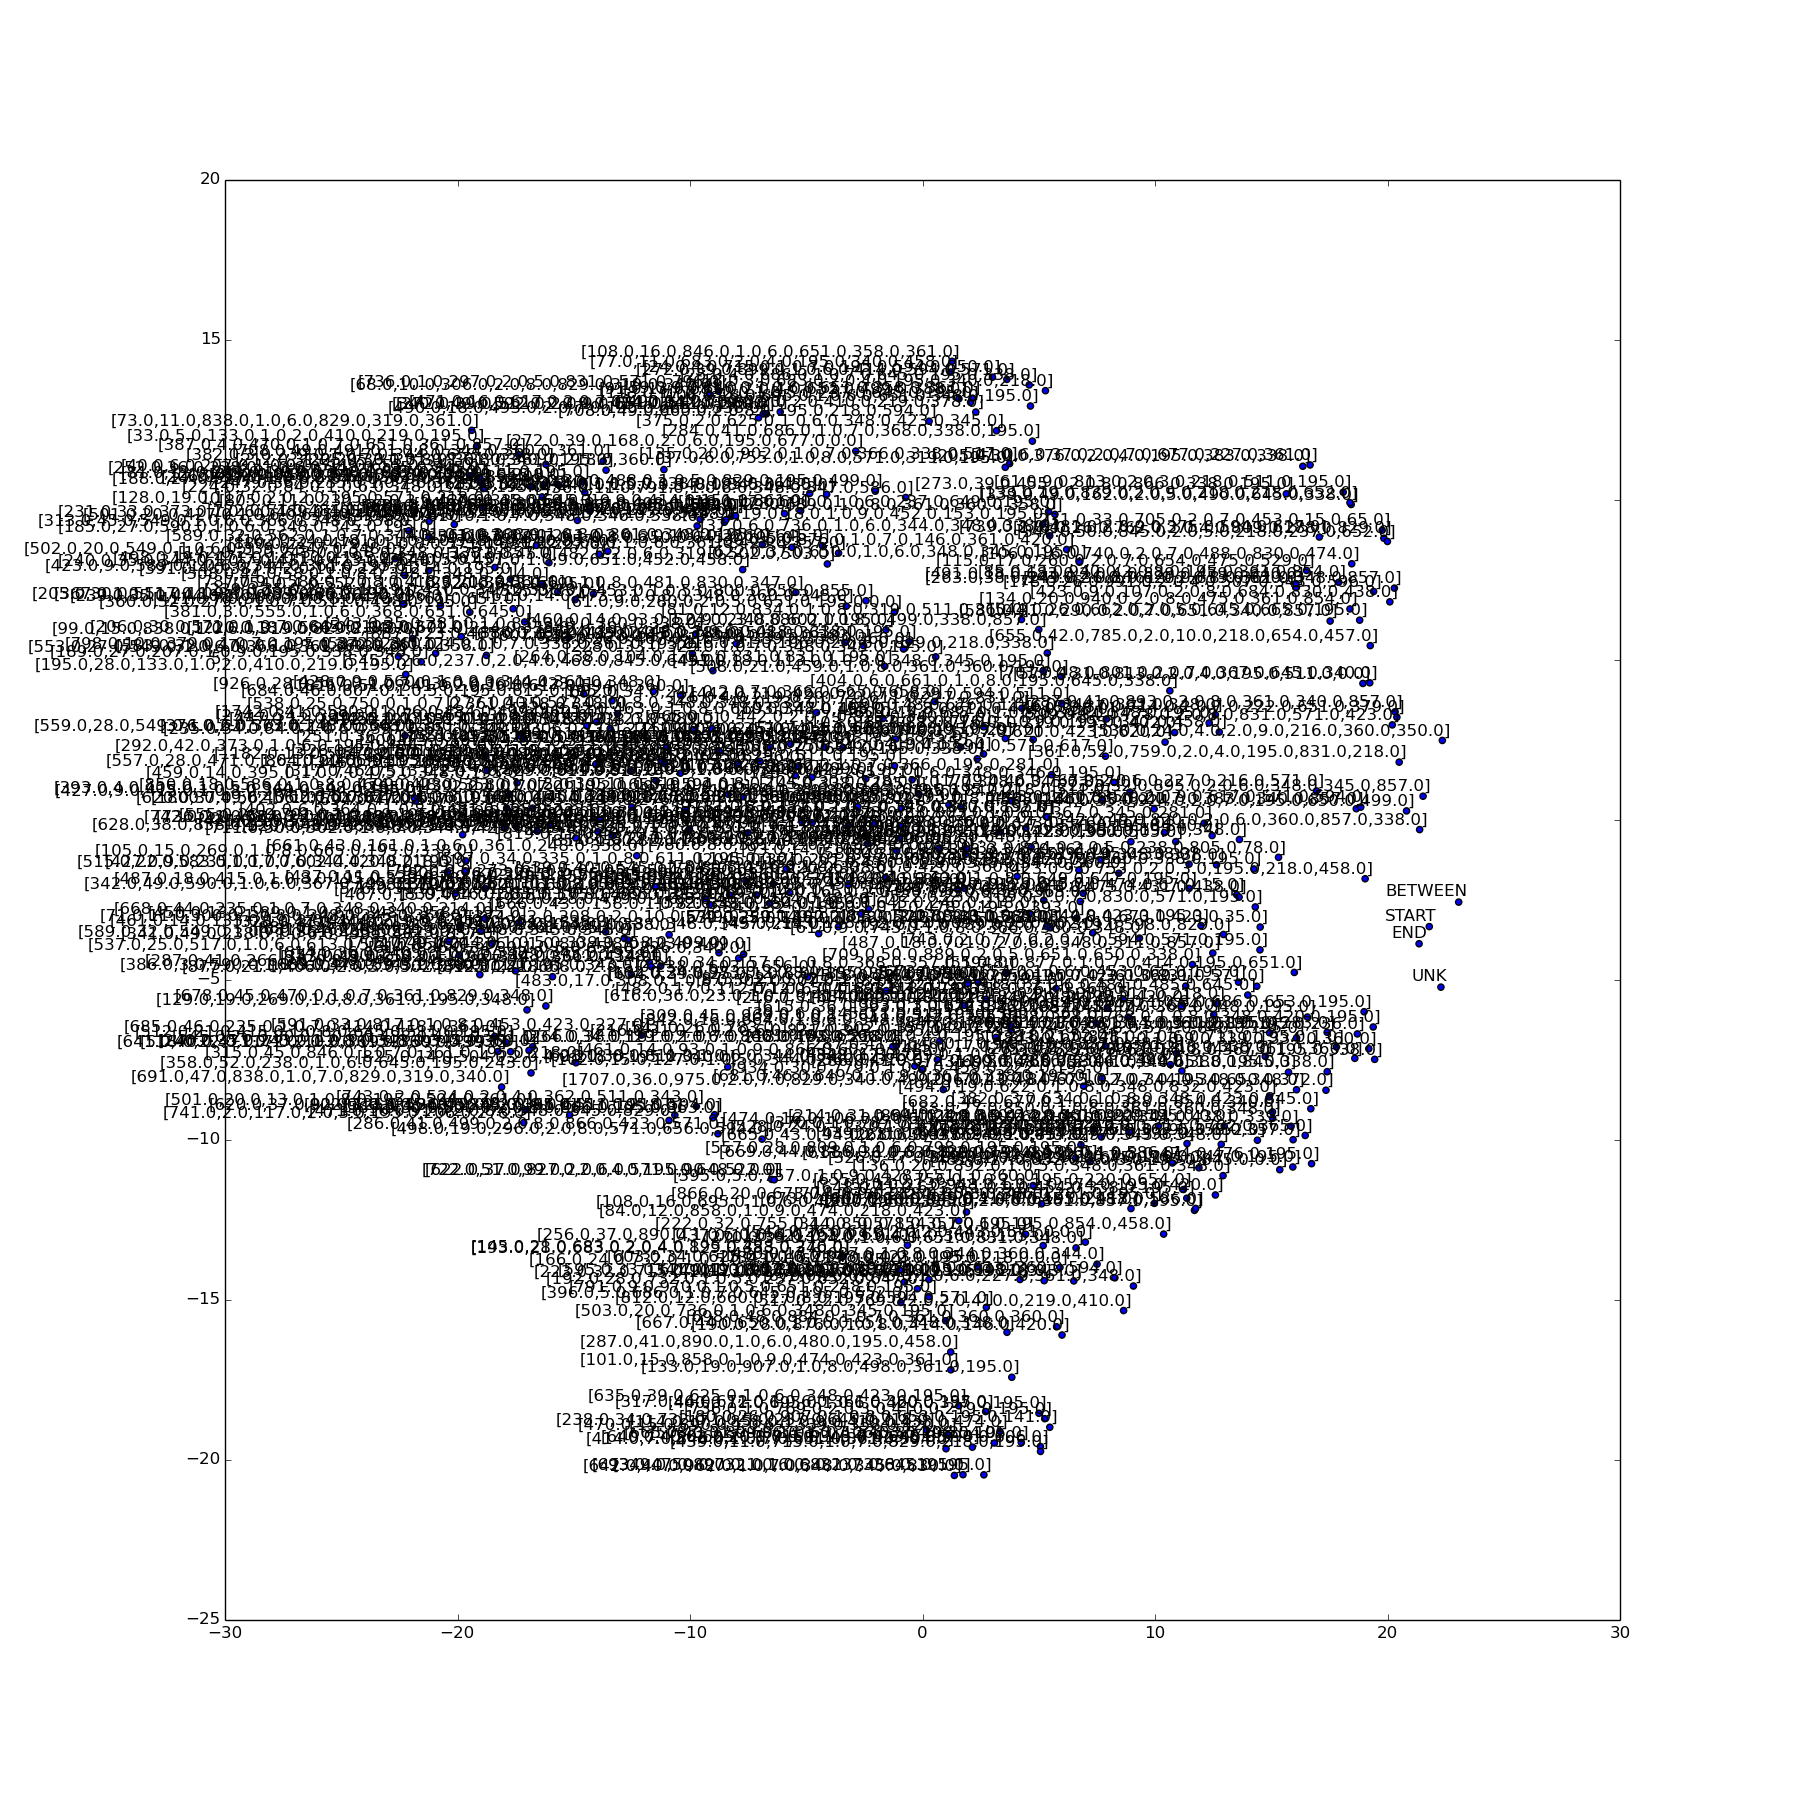
\includegraphics[width=2.5in]{../Figures/visualisation.png}
\caption{A result from the word2vec using the sequences as labels.}
\label{fig:word2vec}
\end{figure}

\subsection{DBSCAN}
In the previous section, we described how to make our data less spars and find relations between words in sequences. \\
Because we have mostly unique events due to the high dimensionality, we clustered the data before we applied the word2vec strategy. \\
We applied the DBSCAN clustering method. It is a density based clustering method which finds core samples when a certain amount of other samples are in their vicinity. When samples are not part of a cluster, they are normally treated as noise in DBSCAN. 

\begin{figure}[H]
\centering
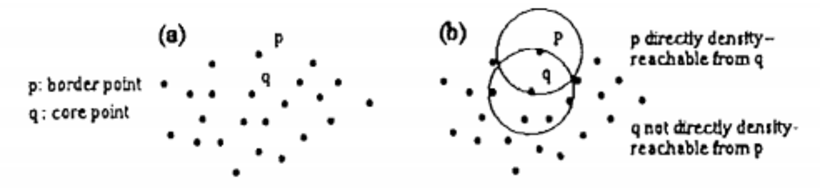
\includegraphics[width=2.5in]{../Figures/dbscan.pdf}
\caption{How a core sample is found based on his vicinity.}
\label{fig:word2vec}
\end{figure}

After we found the clusters, we can approximate each status with their closest core sample. To find the closest core sample, we make a k-d tree\cite{13b}. When the status is seen as noise by DBSCAN, we keep the same status because in medical data outliers are important. \\
To initialize DBSCAN we need to chose two parameters: eps and minSamples. MinSamples is chosen accordingly on how much you want to generalize the data. The higher minSamples, the harder it is to get core samples. Eps is chosen based on the method explained in \cite{13c}.    

\begin{figure}[H]
\centering
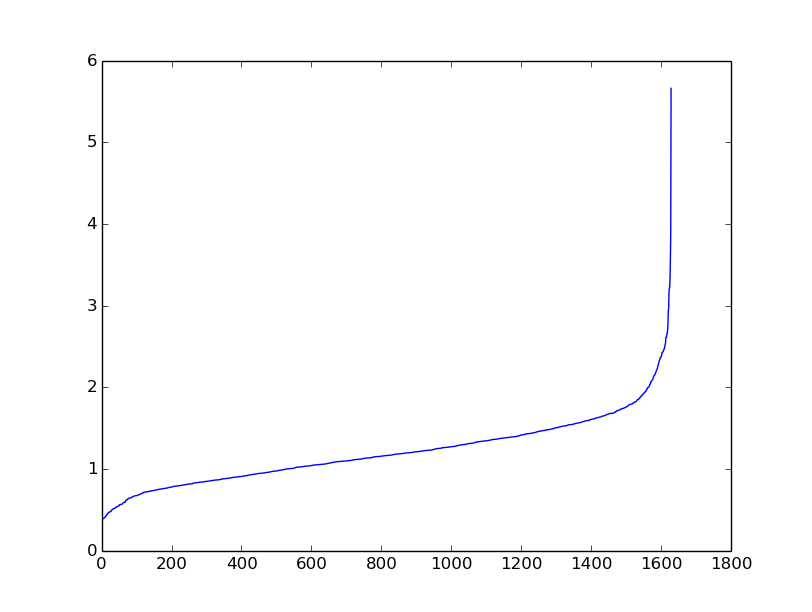
\includegraphics[width=2.5in]{../Figures/eps.png}
\caption{The knick in the figure is how eps is chosen.}
\label{fig:word2vec}
\end{figure}

\section{Experiments}
The effect of the preprocessing can only be validated when the sequence labeling method is worked out. \\
Some possible experiments to validate the clustering are to find common cold diagnoses and see if they match with the cold season. Same can be done for other season related diseases. \\
To test the embedding, we could try to find diagnoses which are closely related to each other. These should be closely to each other in the embedding space.

\section{Future Work}
Until now we described and implemented a method to generalize our dataset and find connections between events. Those results can be used to feed into the LSTM network to label the sequences. With the learned model and the embedding matrix, we can also handle unseen events by looking for the k-nearest neighbors of this unseen event and base our results on the findings of those neighbors. The above improvements will be implemented before the summer of 2016.




% An example of a double column floating figure using two subfigures.
% (The subfig.sty package must be loaded for this to work.)
% The subfigure \label commands are set within each subfloat command,
% and the \label for the overall figure must come after \caption.
% \hfil is used as a separator to get equal spacing.
% Watch out that the combined width of all the subfigures on a 
% line do not exceed the text width or a line break will occur.
%
%\begin{figure*}[!t]
%\centering
%\subfloat[Case I]{\includegraphics[width=2.5in]{box}%
%\label{fig_first_case}}
%\hfil
%\subfloat[Case II]{\includegraphics[width=2.5in]{box}%
%\label{fig_second_case}}
%\caption{Simulation results for the network.}
%\label{fig_sim}
%\end{figure*}
%
% Note that often IEEE papers with subfigures do not employ subfigure
% captions (using the optional argument to \subfloat[]), but instead will
% reference/describe all of them (a), (b), etc., within the main caption.
% Be aware that for subfig.sty to generate the (a), (b), etc., subfigure
% labels, the optional argument to \subfloat must be present. If a
% subcaption is not desired, just leave its contents blank,
% e.g., \subfloat[].


% An example of a floating table. Note that, for IEEE style tables, the
% \caption command should come BEFORE the table and, given that table
% captions serve much like titles, are usually capitalized except for words
% such as a, an, and, as, at, but, by, for, in, nor, of, on, or, the, to
% and up, which are usually not capitalized unless they are the first or
% last word of the caption. Table text will default to \footnotesize as
% IEEE normally uses this smaller font for tables.
% The \label must come after \caption as always.
%
%\begin{table}[!t]
%% increase table row spacing, adjust to taste
%\renewcommand{\arraystretch}{1.3}
% if using array.sty, it might be a good idea to tweak the value of
% \extrarowheight as needed to properly center the text within the cells
%\caption{An Example of a Table}
%\label{table_example}
%\centering
%% Some packages, such as MDW tools, offer better commands for making tables
%% than the plain LaTeX2e tabular which is used here.
%\begin{tabular}{|c||c|}
%\hline
%One & Two\\
%\hline
%Three & Four\\
%\hline
%\end{tabular}
%\end{table}


% Note that the IEEE does not put floats in the very first column
% - or typically anywhere on the first page for that matter. Also,
% in-text middle ("here") positioning is typically not used, but it
% is allowed and encouraged for Computer Society conferences (but
% not Computer Society journals). Most IEEE journals/conferences use
% top floats exclusively. 
% Note that, LaTeX2e, unlike IEEE journals/conferences, places
% footnotes above bottom floats. This can be corrected via the
% \fnbelowfloat command of the stfloats package.




\section{Conclusion}
It is not possible to conclude if the preprocessing works because the sequence labeling method is not implemented yet. 




\begin{thebibliography}{9}

\bibitem{1}
  Henikoff, S. and Henikoff, J. G. (1997), Embedding strategies for effective use of information from multiple sequence alignments. Protein Science, 6: 698–705. doi:10.1002/pro.5560060319
  
\bibitem{2}
	Gabriela Hristescu and Martin Farach-Colton, Cluster-preserving embedding of proteins
	
\bibitem{3}
Dekang Lin. 1996. On the structural complexity of natural language sentences. In Proceedings of the 16th conference on Computational linguistics - Volume 2 (COLING '96), Vol. 2. Association for Computational Linguistics, Stroudsburg, PA, USA, 729-733. DOI=http://dx.doi.org/10.3115/993268.993295

\bibitem{4}
Yoav Goldberg and Omer Levy, word2vec Explained:deriving Mikolov et al.'s negative-sampling word-embedding method

\bibitem{5}
Razan Paul and Abu Sayed Md. Latiful Hoque, Clustering medical data to predict the likelihood of diseases

\bibitem{6} 
P. Kalyani, Approaches to Partition Medical Data using Clustering Algorithms

\bibitem{7}
Pedro Domingos, A Few Useful Things to Know about Machine Learning

\bibitem{8}
Varun Kunmar et al., Outlier Mining in Medical Databases: An Application of Data Mining
in Health Care Management to Detect Abnormal Values Presented In
Medical Databases 

\bibitem{9}
Razvan Pascanu et al., On the difficulty of training recurrent neural networks

\bibitem{10}
Andrew Gelman and Jennifer Hill, Data Analysis using Regression and Multilevel/Hierarchical Models


\bibitem{11}
Eamonn Keogh and Abdullah Mueen, Curse of Dimensionality 

\bibitem{12}
Alex Graves, Supervised Sequence Labeling with Recurrent Neural Networks

\bibitem{13a}
Tomas Mikolov et al., Efficient Estimation of Word Representations in Vector Space

\bibitem{13}
Tomas Mikolov et al., Distributed Representations of Words and Phrases
and their Compositionality

\bibitem{13b}
Freidman, J. H.; Bentley, J. L.; Finkel, R. A. (1977). "An Algorithm for Finding Best Matches in Logarithmic Expected Time". ACM Transactions on Mathematical Software 3 (3): 209. doi:10.1145/355744.355745.

\bibitem{13c}
http://biocomp.cnb.csic.es/~coss/Docencia/ADAM/Notes/ClusteringSlides.pdf

\bibitem{14}
N. Karthikeyani Visalakshi and K. Thangavel, Impact of Normalization in Distributed K-Means Clustering

\bibitem{15} 
http://www.faqs.org/faqs/ai-faq/neural-nets/part2/

\end{thebibliography}






% that's all folks
\end{document}